\chapter{As bactérias e a resistência aos antibióticos}\label{ch:g11:antibiotic-resistance}

Em 1941 um policial que morria de uma septicemia causada por um
arranhão recebeu as primeiras doses de penicilina jamais usadas num
paciente. Ele se recuperou em poucos dias --- e recaiu e morreu quando
acabou o estoque, extraído a duras penas de um bolor. Em uma década a
penicilina era fabricada em toneladas e infecções que matavam havia
milênios passaram a ser curáveis numa semana. Em duas décadas, as
bactérias em que a penicilina já não tocava eram comuns em todos os
hospitais. Este capítulo trata do porquê: como as bactérias variam,
como um \omterm{def:g11:antibiotic-resistance:antibiotic}{antibiótico} as separa, e como a aritmética de uma população de
bilhões transforma uma \omterm{def:g11:mutations:mutation}{mutação} rara num problema de enfermaria inteira.

\begin{omfigure}
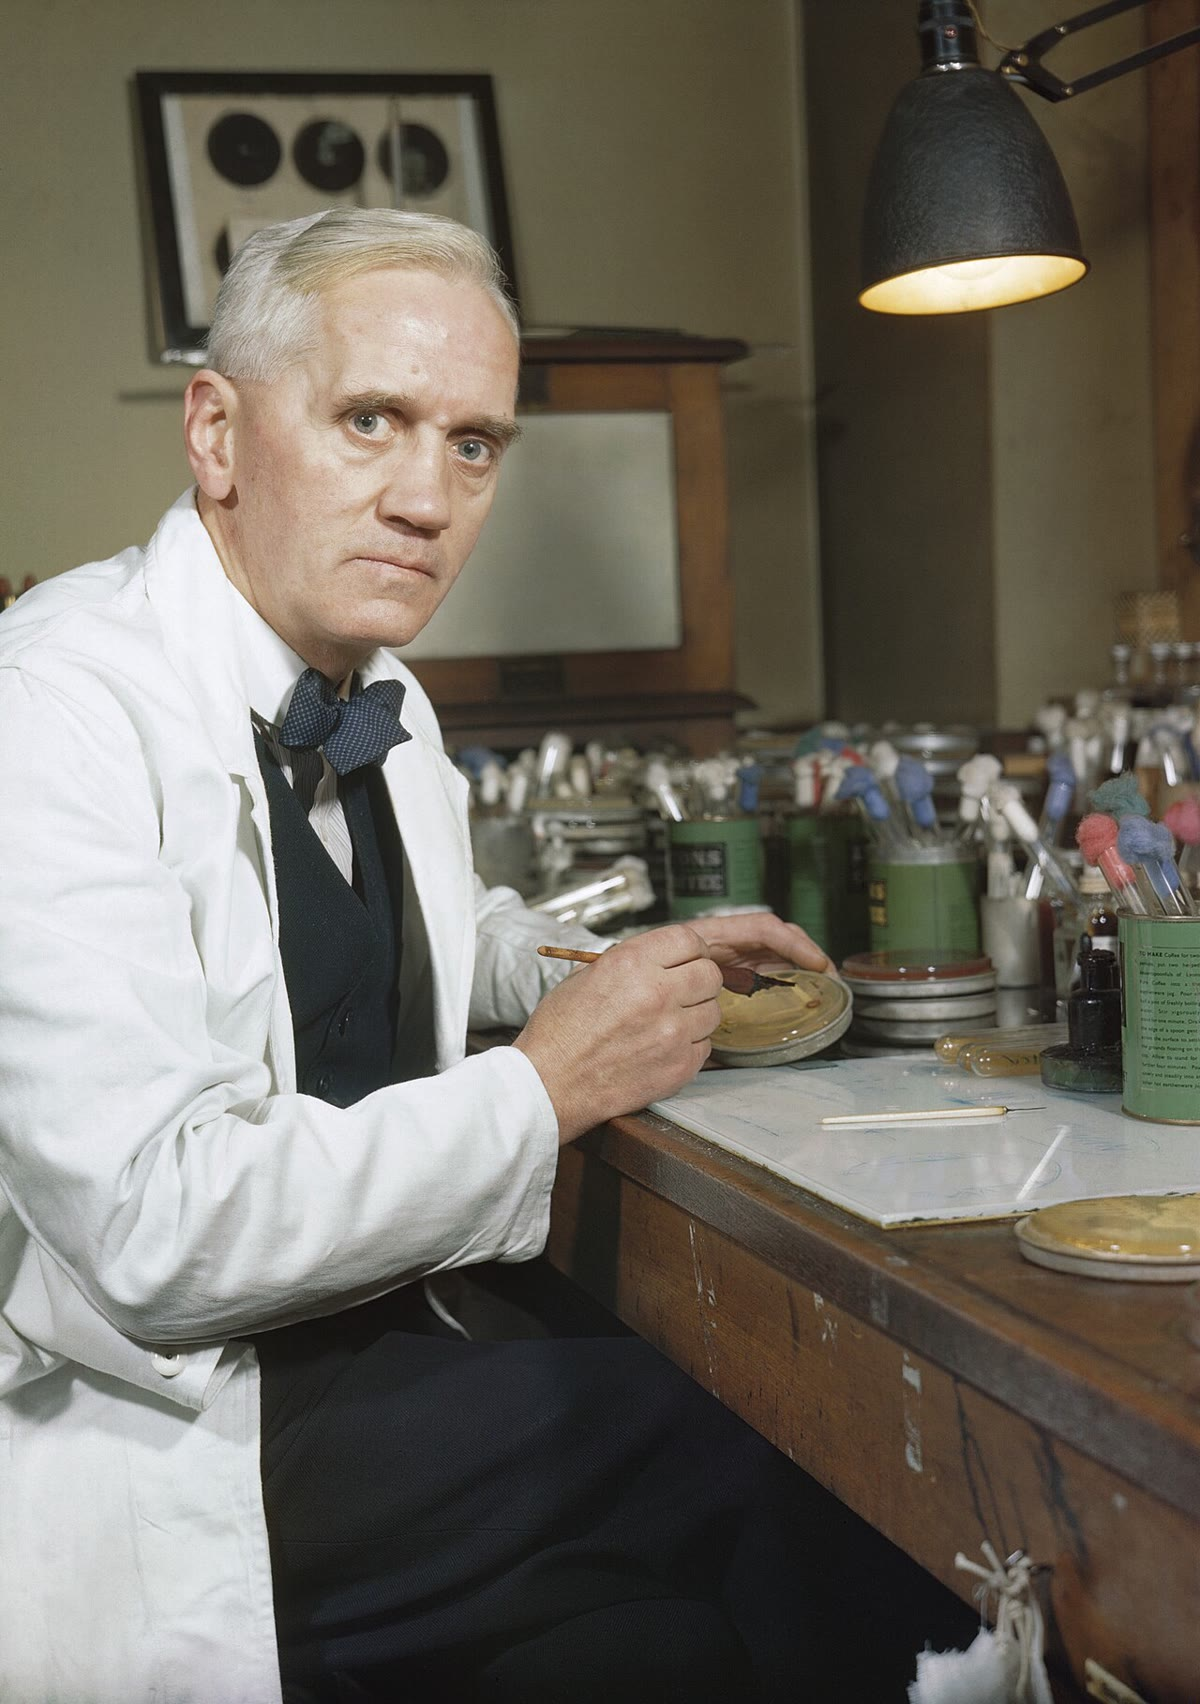
\includegraphics[width=0.4\linewidth]{images/book2/fleming.jpg}

{\small Alexander Fleming em sua bancada em 1943, com as placas de cultura em que, quinze anos antes, ele tinha notado um bolor limpando as bactérias em volta dele. Fotografia, Imperial War Museums, domínio público.}
\end{omfigure}

\section{Como as bactérias variam}

\begin{proposition}[Reprodução e variação nas bactérias]\label{prop:g11:antibiotic-resistance:variation}
Uma bactéria se reproduz dividindo-se em duas depois de copiar o
\omterm{def:g11:cell-cycle-mitosis:chromosome}{cromossomo} único dela: as filhas são, tirando os erros de cópia,
geneticamente idênticas à mãe --- um \emph{clone}. Num meio rico, uma
divisão a cada 20 minutos transforma uma \omterm{def:g10:cells-common-unit:cell}{célula} em um bilhão em dez
horas. A variação genética do clone vem de duas fontes:
\begin{itemize}
  \item as \emph{mutações} (\cref{ch:g11:mutations}), raras por
        divisão, mas frequentes numa população de bilhões;
  \item a \emph{transferência horizontal de genes}\index{transferência horizontal de genes}:
        \omterm{def:g10:universal-dna:information}{DNA} recebido de outra bactéria, da mesma \omterm{def:g10:biodiversity-scales:species}{espécie} ou de outra,
        na maioria das vezes como um \emph{plasmídeo} --- um pequeno
        círculo de \omterm{def:g10:universal-dna:information}{DNA}, separado do \omterm{def:g11:cell-cycle-mitosis:chromosome}{cromossomo}, que carrega alguns
        \omterm{def:g10:universal-dna:gene}{genes} e consegue passar de \omterm{def:g10:cells-common-unit:cell}{célula} a \omterm{def:g10:cells-common-unit:cell}{célula} por uma ponte de
        membrana.
\end{itemize}
\end{proposition}
\admitted

\begin{omfigure}
\begin{tikzpicture}[font=\small, >=Stealth]
  % donor
  \draw[thick, fill=omDef!10, rounded corners=12pt] (0,0) rectangle (3,1.5);
  \draw[thick, omDef] (0.4,0.75) .. controls (0.6,1.3) and (2.4,1.3) .. (2.6,0.75) .. controls (2.4,0.2) and (0.6,0.2) .. (0.4,0.75);
  \draw[thick, omThm, fill=omThm!20] (2.2,1.15) circle (0.22);
  \node[anchor=north] at (1.5,-0.1) {doadora: tem o plasmídeo};
  % recipient
  \draw[thick, fill=omDef!10, rounded corners=12pt] (5,0) rectangle (8,1.5);
  \draw[thick, omDef] (5.4,0.75) .. controls (5.6,1.3) and (7.4,1.3) .. (7.6,0.75) .. controls (7.4,0.2) and (5.6,0.2) .. (5.4,0.75);
  \node[anchor=north] at (6.5,-0.1) {receptora};
  % bridge
  \draw[thick, fill=omProp!30] (3,0.55) rectangle (5,0.95);
  \draw[->, thick, omThm] (3.1,0.75) -- (4.9,0.75);
  \node[anchor=north, font=\scriptsize] at (4,-0.6) {uma cópia do plasmídeo atravessa a ponte};
  % result
  \draw[->, thick] (8.4,0.75) -- (9.2,0.75);
  \draw[thick, fill=omDef!10, rounded corners=12pt] (9.5,0) rectangle (12.5,1.5);
  \draw[thick, omDef] (9.9,0.75) .. controls (10.1,1.3) and (11.9,1.3) .. (12.1,0.75) .. controls (11.9,0.2) and (10.1,0.2) .. (9.9,0.75);
  \draw[thick, omThm, fill=omThm!20] (11.7,1.15) circle (0.22);
  \node[anchor=north, align=center] at (11,-0.1) {a receptora agora carrega\\ os genes do plasmídeo};
  \node[anchor=west, font=\scriptsize, omDef] at (0.2,1.75) {cromossomo};
  \node[anchor=west, font=\scriptsize, omThm] at (2.5,1.75) {plasmídeo};
\end{tikzpicture}

{\small A transferência horizontal. Um plasmídeo --- um pequeno círculo
de \omterm{def:g10:universal-dna:information}{DNA} que pode carregar um \omterm{def:g10:universal-dna:gene}{gene} de resistência --- é copiado através
de uma ponte de uma bactéria para outra, que não precisa ser da mesma
\omterm{def:g10:biodiversity-scales:species}{espécie}. A receptora, e todos os descendentes dela, ganham o \omterm{def:g10:universal-dna:gene}{gene} numa
única etapa.}
\end{omfigure}

\begin{example}[A aritmética de uma população]\label{ex:g11:antibiotic-resistance:arithmetic}
Uma \omterm{def:g11:mutations:mutation}{mutação} de resistência surge cerca de uma vez em $10^8$ divisões.
Um frasco com $10^9$ bactérias teve, portanto, nas divisões que o
produziram, umas dez mutações dessas; uma ferida infectada ou um
intestino, com $10^{12}$ bactérias, umas dez mil. Toda população grande
de bactérias contém, antes de qualquer \omterm{def:g11:antibiotic-resistance:antibiotic}{antibiótico} ser usado, \omterm{def:g10:cells-common-unit:cell}{células}
resistentes a ele --- as placas de réplica do
\cref{ch:g11:mutations} provaram isso.
\end{example}

\section{Os antibióticos}

\begin{definition}[Antibiótico]\label{def:g11:antibiotic-resistance:antibiotic}
Um \emph{antibiótico}\index{antibiótico} é uma molécula que mata as
bactérias ou interrompe o crescimento delas, em concentrações
inofensivas às \omterm{def:g10:cells-common-unit:cell}{células} do paciente, agindo sobre uma estrutura ou um
processo que as bactérias têm e as \omterm{def:g10:cells-common-unit:cell}{células} humanas não: a penicilina e
os parentes dela bloqueiam a construção da parede bacteriana; a
estreptomicina e a tetraciclina travam o \omterm{def:g10:cells-common-unit:organelle}{ribossomo} bacteriano, que
difere do nosso; outros bloqueiam as \omterm{def:g11:enzymes-and-phenotype:enzyme}{enzimas} bacterianas da \omterm{def:g11:dna-replication:replication}{replicação
do DNA}. A maioria foi encontrada primeiro em bolores e em bactérias do
solo, que os fabricam contra os concorrentes deles. Os antibióticos não
têm efeito nenhum sobre os vírus, que não têm nenhum desses alvos.
\end{definition}

\begin{proposition}[Mecanismos de resistência]\label{prop:g11:antibiotic-resistance:mechanisms}
Uma bactéria é \emph{resistente}\index{resistência a antibióticos} a um
\omterm{def:g11:antibiotic-resistance:antibiotic}{antibiótico} quando cresce em concentrações que detêm os parentes
sensíveis dela. A resistência tem uma base genética de um entre poucos
tipos: um \omterm{def:g10:universal-dna:gene}{gene} de uma \omterm{def:g11:enzymes-and-phenotype:enzyme}{enzima} que destrói o \omterm{def:g11:antibiotic-resistance:antibiotic}{antibiótico} (as
penicilinases cortam a penicilina em duas); uma \omterm{def:g11:mutations:mutation}{mutação} que altera o
alvo do \omterm{def:g11:antibiotic-resistance:antibiotic}{antibiótico} de modo que o medicamento não se ligue mais (uma
\omterm{def:g11:gene-expression:protein}{proteína} ribossômica alterada); uma bomba que expulsa o medicamento;
uma parede que não o deixa entrar. Cada um é um \omterm{def:g10:universal-dna:gene}{alelo} ou um \omterm{def:g10:universal-dna:gene}{gene}, e
cada um é herdado --- verticalmente pelo clone e, quando está num
plasmídeo, horizontalmente pelos vizinhos.
\end{proposition}
\admitted

\begin{method}[Ler um antibiograma]\label{met:g11:antibiotic-resistance:antibiogram}
Um \emph{antibiograma} testa as bactérias de um paciente contra vários
\omterm{def:g11:antibiotic-resistance:antibiotic}{antibióticos} ao mesmo tempo.
\begin{enumerate}
  \item Espalhe as bactérias por igual numa placa; disponha discos de
        papel embebidos cada um em um \omterm{def:g11:antibiotic-resistance:antibiotic}{antibiótico}; incube durante a
        noite.
  \item O \omterm{def:g11:antibiotic-resistance:antibiotic}{antibiótico} se difunde para fora do disco, com a
        concentração caindo com a distância; as bactérias crescem
        formando um tapete, exceto onde a concentração as detém: um
        \emph{halo de inibição} transparente em volta de cada disco.
  \item Meça o diâmetro de cada halo e compare com o limiar
        estabelecido para aquele \omterm{def:g11:antibiotic-resistance:antibiotic}{antibiótico}: um diâmetro acima do
        limiar quer dizer sensível, abaixo dele resistente.
  \item Os maiores halos entre os resultados sensíveis orientam a
        prescrição; um disco sem halo nenhum é um \omterm{def:g11:antibiotic-resistance:antibiotic}{antibiótico} que a
        linhagem ignora.
\end{enumerate}
\end{method}

\begin{omfigure}
\begin{tikzpicture}[font=\small]
  \draw[thick, fill=omProp!12] (0,0) circle (3.7);
  \foreach \a/\r/\l in {90/1.3/A, 162/0.9/B, 234/0.0/C, 306/1.6/D, 18/0.55/E} {
    \begin{scope}[shift={(\a:2.0)}]
      \ifdim \r pt > 0pt \draw[fill=white] (0,0) circle (\r); \fi
      \draw[fill=gray!30] (0,0) circle (0.28);
      \node[font=\scriptsize] at (0,0) {\l};
    \end{scope}
  }
  \node[anchor=west, align=left] at (3.8,1.6) {A: halo de \qty{26}{mm}, limiar 17: sensível};
  \node[anchor=west, align=left] at (3.8,0.9) {B: halo de \qty{18}{mm}, limiar 20: resistente};
  \node[anchor=west, align=left] at (3.8,0.2) {C: sem halo: resistente};
  \node[anchor=west, align=left] at (3.8,-0.5) {D: halo de \qty{32}{mm}, limiar 22: sensível};
  \node[anchor=west, align=left] at (3.8,-1.2) {E: halo de \qty{11}{mm}, limiar 15: resistente};
  \node[anchor=north, align=center] at (0,-3.9) {tapete das bactérias do paciente;\\ discos claros de ágar transparente em volta dos discos de antibiótico};
\end{tikzpicture}

{\small Um antibiograma lido. Cada disco contém um \omterm{def:g11:antibiotic-resistance:antibiotic}{antibiótico}; o halo
transparente é onde as bactérias não conseguiram crescer. Comparados
com o limiar de cada medicamento, os diâmetros classificam a linhagem
como sensível a A e D e resistente a B, C e E.}
\end{omfigure}

\begin{omfigure}
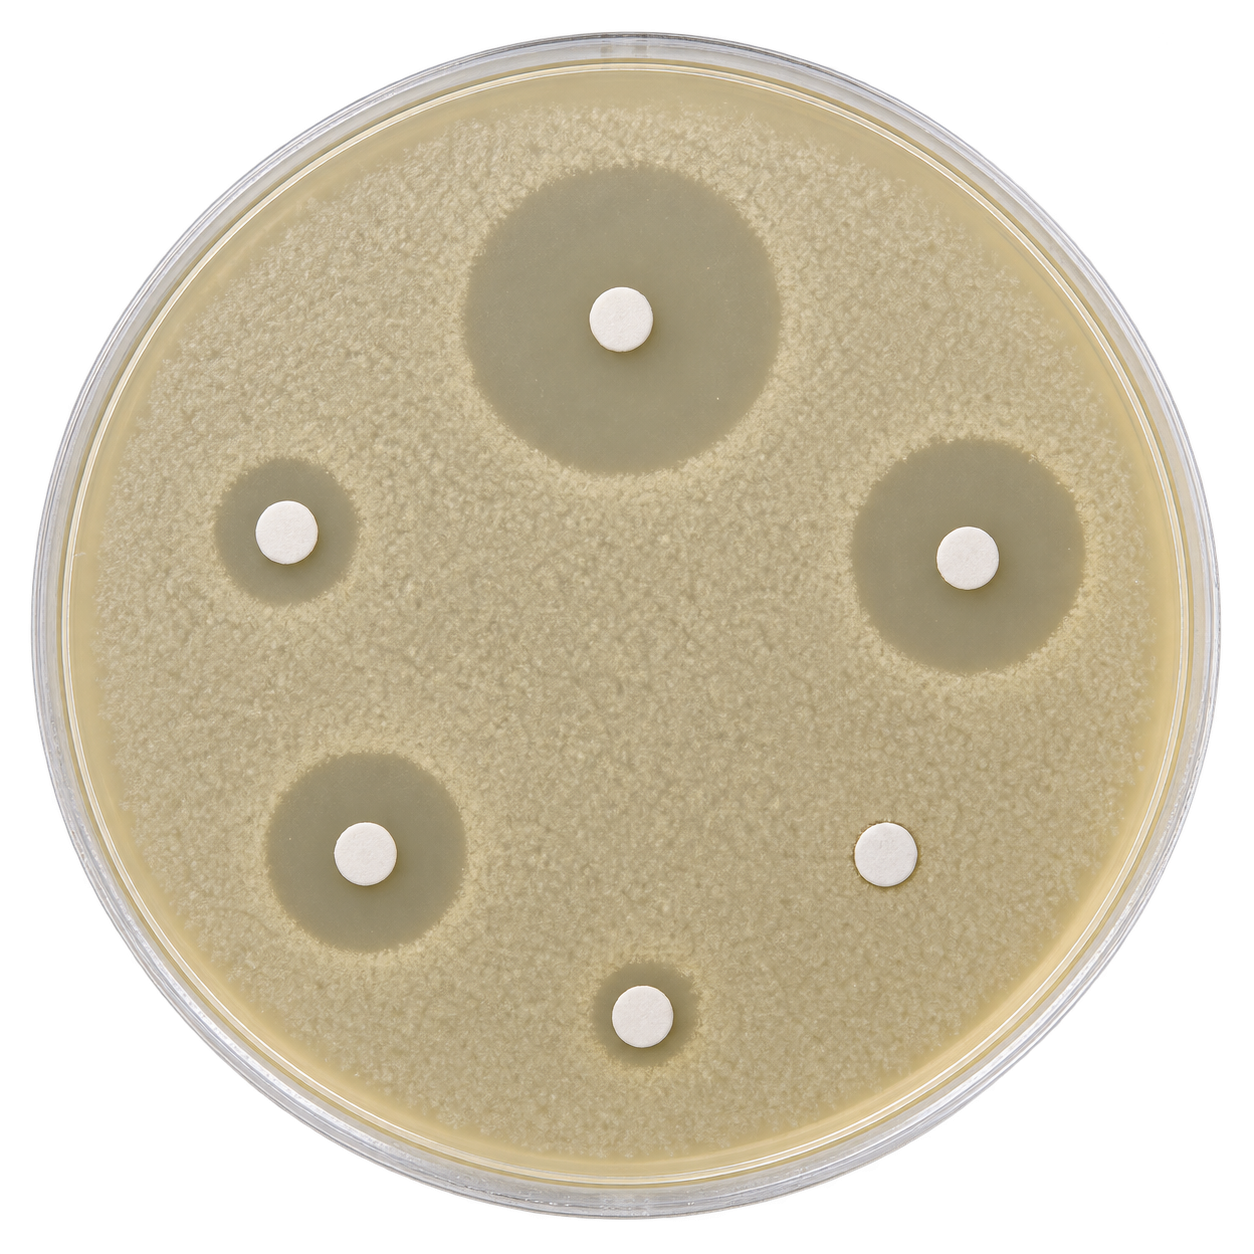
\includegraphics[width=0.44\linewidth]{images/book2/ai/g11-antibiogram-plate.png}

{\small Uma placa de antibiograma depois de uma noite de incubação: um
tapete de bactérias e, em volta de cada disco de \omterm{def:g11:antibiotic-resistance:antibiotic}{antibiótico}, um halo
transparente cujo tamanho mede a sensibilidade da linhagem. Um dos
discos não tem halo.}
\end{omfigure}

\section{Como a resistência se espalha}

\begin{proposition}[A seleção pelo antibiótico]\label{prop:g11:antibiotic-resistance:selection}
Um \omterm{def:g11:antibiotic-resistance:antibiotic}{antibiótico} não cria bactérias resistentes; ele as \emph{seleciona}.
Numa população em que algumas \omterm{def:g10:cells-common-unit:cell}{células} carregam um \omterm{def:g10:universal-dna:gene}{alelo} de resistência,
o medicamento mata ou detém a maioria sensível e deixa as poucas
resistentes se multiplicarem sem concorrência: em poucos dias a
população é resistente. Quanto mais um \omterm{def:g11:antibiotic-resistance:antibiotic}{antibiótico} é usado --- em
pacientes, em animais, no ambiente ---, mais vezes essa separação
acontece, e mais resistentes ficam as bactérias de um hospital, de uma
fazenda ou de um país. Um tratamento incompleto, que mata as \omterm{def:g10:cells-common-unit:cell}{células}
mais sensíveis e poupa as menos sensíveis, é o que seleciona com mais
eficiência.
\end{proposition}
\begin{proof}[Evidências]
As placas de réplica de Lederberg mostraram as \omterm{def:g10:cells-common-unit:cell}{células} resistentes
presentes antes da exposição. Culturas mantidas uma semana em
concentrações crescentes de um \omterm{def:g11:antibiotic-resistance:antibiotic}{antibiótico} terminam resistentes a cem
vezes a dose inicial, e a resistência delas é herdada e mapeada em
mutações específicas. Os países que mais usam \omterm{def:g11:antibiotic-resistance:antibiotic}{antibióticos} por pessoa
têm as maiores proporções de linhagens resistentes; enfermarias que
reduzem o uso veem a resistência cair ao longo de meses. Uma linhagem
da bactéria da pele \emph{Staphylococcus aureus} resistente à
penicilina apareceu quatro anos depois da introdução do medicamento e
hoje responde pela maior parte das linhagens hospitalares; a linhagem
resistente ao medicamento substituto veio dois anos depois dele.
\end{proof}

\begin{omfigure}
\begin{tikzpicture}
\begin{axis}[
  width=0.88\linewidth, height=5.8cm,
  axis x line=bottom, axis y line=left,
  xmin=0, xmax=6, ymin=0, ymax=110,
  xlabel={dias de tratamento}, ylabel={bactérias (\% do inicial)},
  xlabel style={font=\small, at={(axis description cs:0.5,-0.12)}, anchor=north},
  ylabel style={font=\small},
  tick label style={font=\small}, xtick={0,1,2,3,4,5,6}, ytick={0,25,50,75,100},
  legend style={at={(0.5,-0.3)}, anchor=north, legend columns=3, font=\small, draw=none},
  clip=false,
]
\addplot[thick, omDef] coordinates {(0,100) (0.5,45) (1,15) (1.5,5) (2,1.5) (3,0.2) (4,0.05) (5,0.01) (6,0)};
\addplot[thick, omThm] coordinates {(0,0.001) (1,0.01) (2,0.1) (3,1) (4,8) (5,40) (6,100)};
\addplot[thick, omMeth, dashed] coordinates {(0,100) (0.5,45) (1,15) (1.5,5) (2,1.5) (3,1.2) (4,9) (5,48) (6,100)};
\legend{células sensíveis, células resistentes (uma em $10^5$), total se o tratamento parar no dia 3}
\end{axis}
\end{tikzpicture}

{\small Seleção durante um tratamento com \omterm{def:g11:antibiotic-resistance:antibiotic}{antibiótico}. As \omterm{def:g10:cells-common-unit:cell}{células}
sensíveis (em azul) são mortas em poucos dias; as poucas resistentes
(em vermelho) se multiplicam sem oposição e, no fim da semana, formam a
população inteira. Se o paciente parar no dia 3, os sobreviventes
voltam a crescer --- agora quase todos resistentes.}
\end{omfigure}

\begin{example}[De uma célula a uma enfermaria]\label{ex:g11:antibiotic-resistance:ward}
Um paciente tratado com penicilina carrega, entre $10^{10}$ bactérias,
uma centena de resistentes. Em três dias as sensíveis sumiram e o clone
resistente tomou o lugar delas: $10^{10}$ \omterm{def:g10:cells-common-unit:cell}{células} resistentes. Nas mãos
de um enfermeiro, na grade de uma cama, no paciente seguinte, o clone
continua --- e, se o \omterm{def:g10:universal-dna:gene}{gene} de resistência dele estiver num plasmídeo,
ele o entrega a outras \omterm{def:g10:biodiversity-scales:species}{espécies} pelo caminho. Nada nessa sequência
exigiu que o \omterm{def:g11:antibiotic-resistance:antibiotic}{antibiótico} agisse sobre o \omterm{def:g10:universal-dna:information}{DNA}; ele apenas retirou a
concorrência.
\end{example}

\section{Manter os antibióticos funcionando}

\begin{proposition}[Consequências e respostas]\label{prop:g11:antibiotic-resistance:consequences}
As infecções resistentes são mais longas, mais caras e mais vezes
fatais; algumas linhagens já resistem a todos os medicamentos
disponíveis. Como a resistência é impulsionada pelo uso, a resposta é
usar \omterm{def:g11:antibiotic-resistance:antibiotic}{antibióticos} menos e melhor: só para infecções bacterianas (nunca
para resfriados e gripes virais), escolhidos depois de um antibiograma
sempre que possível, na dose completa e pelo tratamento completo, com o
medicamento de espectro mais estreito que funcione; limitar o uso deles
na criação de animais; prevenir infecções (higiene, vacinação) para que
menos tratamentos sejam necessários; e isolar nos hospitais os
portadores de linhagens resistentes. \omterm{def:g11:antibiotic-resistance:antibiotic}{Antibióticos} novos compram tempo;
a aritmética da seleção garante que a resistência a cada um vai
aparecer.
\end{proposition}
\admitted

\begin{remark}[Evolução em uma semana]\label{rem:g11:antibiotic-resistance:evolution}
A \omterm{def:g11:mutations:mutation}{mutação} fornecendo variação ao acaso, o ambiente separando-a, os
descendentes dos sobreviventes herdando a diferença: as bactérias deste
capítulo percorrem, em uma semana, o processo que o último ano vai
descrever ao longo de milhões de anos para as baleias e os carvalhos. A
resistência aos \omterm{def:g11:antibiotic-resistance:antibiotic}{antibióticos} é a evolução por seleção natural observada
em tempo real, com os seres humanos como agente selecionador --- e a
demonstração mais clara de que o processo não é uma teoria sobre o
passado, e sim um fato sobre qualquer população que varie e se
reproduza.
\end{remark}

\section{Exercícios}

\begin{exercise}[$\star$]\label{exo:g11:antibiotic-resistance:1}
Cite as duas fontes de variação genética numa população de bactérias.
\end{exercise}

\begin{exercise}[$\star$]\label{exo:g11:antibiotic-resistance:2}
O que é um \omterm{def:g11:antibiotic-resistance:antibiotic}{antibiótico}, e por que ele prejudica as bactérias mas não as
\omterm{def:g10:cells-common-unit:cell}{células} do paciente? Por que ele é inútil contra um resfriado?
\end{exercise}

\begin{exercise}[$\star$]\label{exo:g11:antibiotic-resistance:3}
Dê três mecanismos pelos quais uma bactéria pode resistir a um \omterm{def:g11:antibiotic-resistance:antibiotic}{antibiótico}.
\end{exercise}

\begin{exercise}[$\star$]\label{exo:g11:antibiotic-resistance:4}
Na figura do antibiograma, um disco F novo dá um halo de \qty{20}{mm}
com um limiar de \qty{18}{mm}. Sensível ou resistente? Que \omterm{def:g11:antibiotic-resistance:antibiotic}{antibiótico}
você prescreveria entre A e F?
\end{exercise}

\begin{exercise}[$\star$]\label{exo:g11:antibiotic-resistance:5}
Um \omterm{def:g11:antibiotic-resistance:antibiotic}{antibiótico} causa mutações de resistência? Justifique com o
experimento do \cref{ch:g11:mutations}.
\end{exercise}

\begin{exercise}[$\star\star$]\label{exo:g11:antibiotic-resistance:6}
Partindo de uma bactéria que se divide a cada 20 minutos, quantas
existem depois de 10 horas? Se a resistência surge uma vez a cada
$10^8$ divisões, quantas \omterm{def:g10:cells-common-unit:cell}{células} resistentes a cultura provavelmente
contém?
\end{exercise}

\begin{exercise}[$\star\star$]\label{exo:g11:antibiotic-resistance:7}
A partir da figura da seleção, em que dia as \omterm{def:g10:cells-common-unit:cell}{células} resistentes se
tornam a maioria do total? Qual é a população total no dia 6 no caso
tracejado, e do que ela é feita?
\end{exercise}

\begin{exercise}[$\star\star$]\label{exo:g11:antibiotic-resistance:8}
Explique por que um \omterm{def:g10:universal-dna:gene}{gene} de resistência num plasmídeo se espalha mais
depressa que um no \omterm{def:g11:cell-cycle-mitosis:chromosome}{cromossomo}.
\end{exercise}

\begin{exercise}[$\star\star$]\label{exo:g11:antibiotic-resistance:9}
Um paciente se sente melhor depois de três dias de um tratamento de
sete dias e para. Explique, com a figura, o que acontece nos dias
seguintes e por que a recaída é mais difícil de tratar.
\end{exercise}

\begin{exercise}[$\star\star$]\label{exo:g11:antibiotic-resistance:10}
Por que a proporção de linhagens resistentes é maior nos hospitais que
na população geral?
\end{exercise}

\begin{exercise}[$\star\star$]\label{exo:g11:antibiotic-resistance:11}
Explique por que uma \omterm{def:g11:mutations:mutation}{mutação} que altera uma \omterm{def:g11:gene-expression:protein}{proteína} ribossômica pode
tornar uma bactéria resistente à estreptomicina, e por que uma bactéria
dessas muitas vezes cresce um pouco mais devagar que os parentes
sensíveis dela.
\end{exercise}

\begin{exercise}[$\star\star\star$]\label{exo:g11:antibiotic-resistance:12}
Dois \omterm{def:g11:antibiotic-resistance:antibiotic}{antibióticos} de alvos diferentes são dados juntos. Estime a
probabilidade de uma \omterm{def:g10:cells-common-unit:cell}{célula} ser resistente aos dois por mutações
independentes (uma em $10^8$ cada), e explique por que a terapia
combinada é usada contra infecções lentas e longas como a tuberculose.
\end{exercise}

\begin{exercise}[$\star\star\star$]\label{exo:g11:antibiotic-resistance:13}
Uma fazenda acrescenta doses baixas de um \omterm{def:g11:antibiotic-resistance:antibiotic}{antibiótico} à ração dos
animais para acelerar o crescimento. Preveja as consequências para as
bactérias dos animais, para os trabalhadores da fazenda e para a
medicina humana, usando a seleção e a transferência horizontal.
\end{exercise}

\begin{exercise}[$\star\star\star$]\label{exo:g11:antibiotic-resistance:14}
Uma enfermaria reduz à metade as prescrições de \omterm{def:g11:antibiotic-resistance:antibiotic}{antibióticos}; em um ano
a proporção de linhagens resistentes cai. Explique por que a
resistência pode recuar, usando o custo da resistência para a bactéria
e a concorrência.
\end{exercise}

\begin{exercise}[$\star\star\star$]\label{exo:g11:antibiotic-resistance:15}
``As bactérias ficam resistentes porque se acostumam ao \omterm{def:g11:antibiotic-resistance:antibiotic}{antibiótico}.''
Reescreva essa frase corretamente, num parágrafo curto, usando \omterm{def:g11:mutations:mutation}{mutação},
seleção e hereditariedade.
\end{exercise}

\section{Problema: a enfermaria}

\begin{problem}[{Problema de fim de semana --- um surto numa enfermaria
de hospital acompanhado a partir de uma única célula mutante: a
aritmética de uma colônia, um antibiograma lido, um tratamento
interrompido, e a política que interrompe a disseminação}]
\label{pb:g11:antibiotic-resistance:1}
A ferida de um paciente está infectada com $10^{10}$ bactérias de uma
\omterm{def:g10:biodiversity-scales:species}{espécie}. As bactérias se dividem a cada 30 minutos; uma \omterm{def:g11:mutations:mutation}{mutação} que dá
resistência ao \omterm{def:g11:antibiotic-resistance:antibiotic}{antibiótico} amoxicilina acontece uma vez a cada $10^8$
divisões. O \omterm{def:g11:antibiotic-resistance:antibiotic}{antibiótico} mata 90\% das \omterm{def:g10:cells-common-unit:cell}{células} sensíveis a cada 6 horas
e não afeta as \omterm{def:g10:cells-common-unit:cell}{células} resistentes, que continuam se dividindo.

\medskip
\noindent\textbf{Parte I --- Antes do tratamento.}
\begin{enumerate}
  \item Quantas divisões produziram as $10^{10}$ bactérias a partir da
        primeira \omterm{def:g10:cells-common-unit:cell}{célula}? (Conte o número de \omterm{def:g10:cells-common-unit:cell}{células}.)
  \item Estime o número de \omterm{def:g10:cells-common-unit:cell}{células} resistentes presentes antes de
        qualquer \omterm{def:g11:antibiotic-resistance:antibiotic}{antibiótico} ser dado.
  \item Explique por que a infecção do paciente é, apesar disso,
        descrita como ``sensível'' no antibiograma.
  \item O antibiograma mostra halos de \qty{24}{mm} para a amoxicilina
        (limiar 17), \qty{12}{mm} para a eritromicina (limiar 20) e
        nenhum para a penicilina. Interprete os três resultados.
  \item O médico prescreve amoxicilina por 7 dias. Por que não
        penicilina, e por que não o medicamento de maior halo, se
        algum fosse maior?
\end{enumerate}

\medskip
\noindent\textbf{Parte II --- Durante o tratamento.}
\begin{enumerate}[resume]
  \item Quantas \omterm{def:g10:cells-common-unit:cell}{células} sensíveis restam depois de 1 dia? E depois de
        3 dias?
  \item Partindo da resposta da questão 2, quantas \omterm{def:g10:cells-common-unit:cell}{células} resistentes
        existem depois de 1 dia, se elas dobram a cada 30 minutos sem
        limite? (Use $2^{48} \approx \num{2.8e14}$.) Por que esse
        número é irrealista, e o que o limita?
  \item Suponha que o clone resistente fique limitado ao espaço que as
        \omterm{def:g10:cells-common-unit:cell}{células} sensíveis desocupam, de modo que ele não possa passar
        de $10^{10}$. Aproximadamente quando ele preenche esse espaço?
  \item Esboce, ou descreva, as curvas das \omterm{def:g10:cells-common-unit:cell}{células} sensíveis, das
        resistentes e do total ao longo dos 7 dias.
  \item Na verdade o sistema imunológico do paciente elimina os
        últimos poucos milhões de \omterm{def:g10:cells-common-unit:cell}{células} de qualquer tipo em alguns
        dias. Explique por que o desfecho depende de o clone resistente
        crescer mais depressa do que o sistema imunológico o elimina.
\end{enumerate}

\medskip
\noindent\textbf{Parte III --- O tratamento interrompido.}
\begin{enumerate}[resume]
  \item O paciente para depois de 2 dias, sentindo-se bem. Quantas
        \omterm{def:g10:cells-common-unit:cell}{células} sensíveis restam, e que fração da população
        sobrevivente é resistente?
  \item As bactérias voltam a crescer até $10^{10}$ nos dias
        seguintes. Que proporção é agora resistente, se as \omterm{def:g10:cells-common-unit:cell}{células}
        resistentes e as sensíveis crescem à mesma taxa?
  \item O paciente recai e recebe amoxicilina de novo. Preveja o
        resultado.
  \item Um antibiograma da recaída não mostra halo nenhum para a
        amoxicilina. Explique a mudança em relação ao primeiro
        antibiograma.
  \item O \omterm{def:g10:universal-dna:gene}{gene} de resistência está num plasmídeo. Que risco a mais
        isso acrescenta para a enfermaria?
\end{enumerate}

\medskip
\noindent\textbf{Parte IV --- A política da enfermaria.}
A enfermaria trata 400 pacientes por ano com amoxicilina; 30\% das
infecções isoladas na enfermaria são hoje resistentes, contra 5\% na
cidade.
\begin{enumerate}[resume]
  \item Explique a diferença entre a enfermaria e a cidade em termos de
        pressão de seleção.
  \item A enfermaria decide: antibiogramas antes de cada prescrição,
        tratamentos completos, higiene das mãos e isolamento dos
        portadores de linhagens resistentes. Diga sobre que mecanismo
        deste capítulo cada medida age.
  \item Depois de dois anos a resistência na enfermaria é de 12\%.
        Explique por que ela caiu e por que não voltou aos 5\%.
  \item Por que um \omterm{def:g11:antibiotic-resistance:antibiotic}{antibiótico} novo, introduzido na enfermaria, não
        resolveria o problema por mais que alguns anos?
  \item Enuncie o resultado: o número de \omterm{def:g10:cells-common-unit:cell}{células} resistentes que a
        ferida abrigava antes de qualquer medicamento, o dia em que
        elas herdaram a ferida, e o único hábito do paciente que
        transformou uma infecção curável num surto.
\end{enumerate}
\end{problem}
